\chapter{La mesure vue comme stochastique}
\label{chap:measurements-stochastic}

\section{La mesure est une variable aléatoire}

Toutes les grandeurs physiques que l'on peut mesurer en ingénierie, physique, etc. sont soit \textbf{stables}, par exemple les dimensions mécaniques d'une pièce, la masse d'un proton, soit \textbf{variables}, par exemple la vitesse en un point donné d'un fluide turbulent, ou la pression atmosphérique.

Par ailleurs, à toute mesure s'ajoute toujours (sauf exception) une erreur aléatoire inconnue\footnote{si elle était connue alors il s'agirait d'une erreur systématique que nous pourrions éliminer}. Tout simplement parce que l'instrument de mesure lui-même est sensible aux conditions de son utilisation, et est susceptible de donner, pour la même grandeur physique, des mesures légèrement variables. Par exemple, lors de la mesure d'une dimension avec un pied à coulisse, si l'opérateur appuie un peu trop au contact de la pièce, les palpeurs vont se déformer légèrement, élastiquement, conduisant à une mesure qui diffère de la valeur réelle.

De fait, lorsque l'on effectue la mesure d'une grandeur physique, il est exceptionnel d'obtenir une valeur parfaitement stable: soit la grandeur est variable dans le temps, soit l'instrument de mesure est affecté par une erreur aléatoire, soit encore ces effets surviennent simultanément. Il n'y a en fait que lors de comptages d'éléments que les risques d'erreur sont pratiquement nuls (comptage du nombre de pièces dans une boite, par exemple)

Nous considérerons donc, dans ce cours, que le résultat de toute mesure est entaché d'une fluctuation aléatoire \textbf{non prédictible}, et nous allons étudier les caractéristiques statistiques de ces fluctuations.

\section{Définitions}

\subsection{Variable aléatoire}

Considérons une grandeur physique quelconque $X$, que l'on peut mesurer (comme la température). Si, d'une mesure à l'autre, le résultat de la mesure de $X$, noté $x$, varie de manière aléatoire, non prédictible, alors on dira que la variable $X$ est une \textbf{variable de type aléatoire} (VA dans la suite).

En général, on s'intéresse à la valeur moyenne de la VA, et à son écart-type. Pour connaitre ces propriétés statistiques, il faudra faire un grand nombre $N\gg 1$ de mesures individuelles $x_i$, $i=1\dots N$.

\subsection{Variable aléatoire stationnaire}

Si les propriétés statistiques d'une VA - moyenne, écart-type, etc. - ne changent pas au cours du temps, alors cette VA est dite \textbf{stationnaire}.
\begin{description}
\item[Un exemple de VA stationnaire:] le diamètre de pièces mécaniques usinées par une machine-outil;
\item[Un exemple de VA non-stationnaire:] la vitesse du vent au sommet d'une montagne (car les conditions météorologiques évoluent de manière continue).
\end{description}
En fait, il est plus facile d'imaginer des exemples de VA non-stationnaires que le contraire. Une VA stationnaire, souvent, ne l'est que pendant un temps limité. Il suffit que les conditions externes à la mesure changent pour que les propriétés statistiques de la VA changent aussi. Par exemple, toutes les VA météorologiques ne sont que des VA momentanément stationnaires.

\subsection{Variable aléatoire discrète}

Une VA \textbf{discrète} est une VA qui ne peut prendre que des valeurs \textbf{bien déterminées}. Attention, ces valeurs ne sont pas forcément des valeurs entières ! Elles peuvent être le multiple d'une valeur de base, réelle. Par exemple, la VA dont la population est $[0,\pi,2\pi,3\pi,4\pi,5\pi,\cdots,\infty[$ est une VA discrète.

La population d'une VA discrète peut être \textbf{finie ou infinie}. La VA précédente est de population infinie. La VA de population [A,C,G,T] est discrète, de population finie.

\subsection{Variable aléatoire continue}

Une VA continue est une VA qui peut prendre \textbf{n'importe quelle valeur réelle}. La population d'une VA continue est forcément infinie, même si le domaine dans lequel elle prend ses valeurs est borné. Par exemple, la VA associée à la vitesse de n'importe quelle particule dans l'Univers est forcément bornée par l'intervalle $[0,c]$ où $c$ est la vitesse de la lumière dans le vide.

\subsection*{Quelques exemples de variables aléatoires}

Les VA suivantes sont-elles continues ou discrètes ? Stationnaires ? De population limitée ou infinie ?
\begin{itemize}
\item La mesure du diamètre d'un axe avec un pied à coulisse dont la précision est de 0.01 mm. L'axe fait, selon les plans, 20 mm de diamètre. Cette VA est discrète, stationnaire, de population finie;
\item La température du lac Léman, en un point donné, pendant une année complète, avec un thermomètre dont la précision est de 0.1$^\circ$C: cette VA est discrète, non-stationnaire, de population finie;
\item La masse des petits cailloux que l'on s'amuse à jeter dans l'eau, au bord d'une rivière, au lieu de travailler ses cours: cette VA est continue, stationnaire, de population infinie.
\end{itemize}

\section{Universalité des lois de probabilité}

Les probabilités interviennent dans tous les domaines de l'activité humaine (science, technologie, sociologie, etc.). Or, lorsque l'on étudie les répartitions de probabilité des VA associées à n'importe lequel de ces domaines, on retombe \textbf{toujours} sur les mêmes formules ! Seuls les paramètres de ces formules varient d'un cas à l'autre. Le comptage des abeilles qui rentrent à la ruche au coucher du soleil obéit aux mêmes lois que le nombre de voitures dans les bouchons sur l'autoroute à l'heure de pointe du soir, et au nombre de cancers du poumon dus à la pollution engendrée par ce trafic.

Nous allons présenter ici ces différentes lois, en espérant qu'elles puissent vous servir un jour à compter le nombre de papillons dans les champs plutôt que le nombre de balles que tire  une mitrailleuse... bien qu'encore une fois les mathématiques soient les mêmes.

\section{Les distributions de probabilité des variables aléatoires discrètes}

Ce paragraphe constitue un rappel général sur les probabilités des VA discrètes, permettant de mieux appréhender les VA continues, dans les paragraphes suivants.

\subsection{La probabilité discrète}

Soit la VA \textbf{discrète} $X$, mesure d'une certaine grandeur physique. L'ensemble des valeurs possibles de $X$ est donné par la population $\mathcal{P}=[x_1,x_2,x_3,\cdots,x_{N_p}]$, de dimension $N_p$.
% La probabilité $p_k$ que la VA $X$ prenne la valeur $x_k$ est définie par le quotient
%\begin{equation}
%P[X=x_k]=p_k=\frac{\text{nombre de cas où $X=x_k$ parmi tous les résultats possibles}}
%{\text{nombre de résultats possibles}}
%\label{eq:ddlp2}
%\end{equation}
Soit $\mathcal{E}$ un échantillon de $N_m$ mesures de $X$. Dans \textbf{cet} échantillon, la probabilité que $X=x_k$ est naturellement donnée par
\begin{equation}
P_\epsilon[X=x_k]=
\frac{\text{nombre de fois que $X=x_k$}}
{N_m}
\end{equation}
Cependant, tout échantillon est - en principe - unique, c.-à-d. que si on effectue une autre série de $N_m$ mesures, en général le nouvel échantillon sera différent. Par conséquent, pour connaitre la vraie probabilité $p_k$ que $X$ soit égal à la valeur particulière $x_k$, on comprenne qu'il faudrait faire un nombre infini de mesures:
%La probabilité que la VA $X$ possède la valeur précise $x_k$ est alors
\begin{equation}
P[X=x_k]=p_k=\lim_{N_m\rightarrow\infty}
\frac{\text{nombre de fois que $X=x_k$}}{N_m}
\end{equation}

Mais cette formule n'est pas pratique. Il existe une autre façon de déterminer $p_k$, \textbf{si la population est finie}. Il suffit d'identifier, dans le processus qui nous intéresse, de compter toutes les situations où la variable $X$ va prendre la valeur particulière $p_k$, puis de diviser par le nombre de valeurs possibles pour $X$, c.-à-d. par la taille de la population. On aura donc
\begin{equation}
P[X=x_k]=p_k=\frac{\text{nombre total de situations où $X=x_k$}}{N_p}
\label{eq:ddlp2}
\end{equation}

\subsubsection*{Exemple: jet de deux dés à 6 faces}

La mesure est définie par le nombre total de points. La population est donnée par toutes les valeurs possibles, soit.
$$
\mathcal{P}=[2,3,4,5,6,7,8,9,10,11,12]
$$
Pour calculer, $p_k$ on va appliquer la définition de l'équation~(\ref{eq:ddlp2}), et construire le tableau des probabilités:
\begin{center}
\begin{tabular}{clcc}
$x_k$ & combinaisons favorables & nb de c.f. & $p_k$ \\\hline
 2 & [1,1] & 1 & 1/36 \\
 3 & [1,2] [2,1] & 2 & 2/36\\
 4 & [1,3] [2,2] [3,1] & 3 & 3/36 \\
 5 & [1,4] [2,3] [3,2] [4,1] & 4 & 4/36 \\
 6 & [1,5] [2,4] [3,3] [4,2] [5,1] & 5 & 5/36 \\
 7 & [1,6] [2,5] [3,4] [4,3] [5,2] [6,1] & 6 & 6/36 \\
 8 & [2,6] [3,5] [4,4] [5,3] [6,2] & 5 & 5/36 \\
 9 & [3,6] [4,5] [5,4] [6,3] & 4 & 4/36 \\
10 & [4,6] [5,5] [6,4] & 3 & 3/36 \\
11 & [5,6] [6,5] & 2 & 2/36 \\
12 & [6,6] & 1 & 1/36 \\\hline
 & & total 36 & $\sum p_k=1$
\end{tabular}
\end{center}
La distribution de probabilité est montrée en figure~\ref{fig:ddjddd}.
\begin{figure}[h]
   \centering
   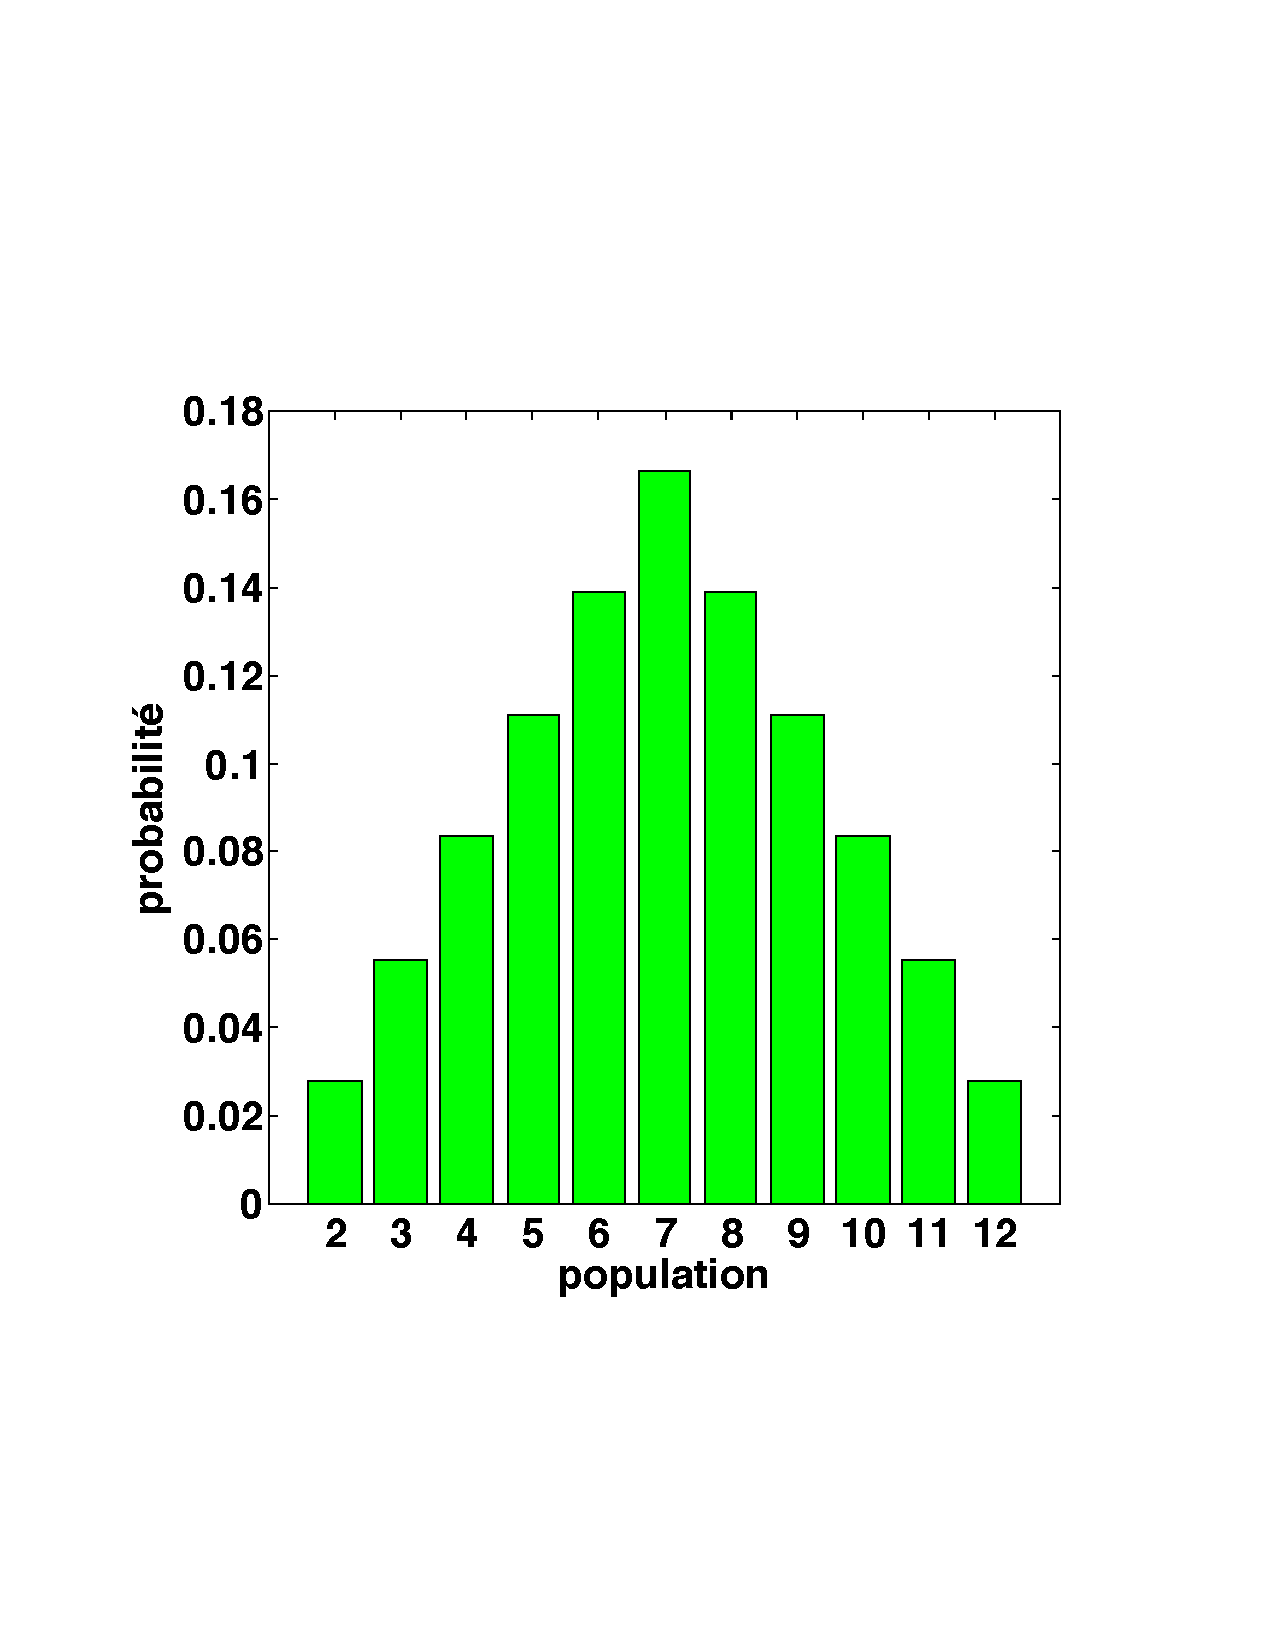
\includegraphics[width=7cm]{assets/figures/Serie2_exe01fig1.pdf}
   \caption{Distribution de probabilité du résultat du jet de 2 dés.}
   \label{fig:ddjddd}
\end{figure}

\subsection{Propriétés de la probabilité discrète}

\begin{itemize}
\item $0\le P[x_k]\le 1$, 0 si l'événement est impossible, 1 si il est certain.
\item $P[x\in\text{population}]=1$ c.-à-d. $\sum_{k=1}^{N_p} p_k=1$
\item $P[x=x_k\ \text{ou}\ x=x_l]=P[x=x_k]+P[x=x_l]=p_k+p_l$
\item si x et y sont deux VA discrètes indépendantes, de populations identiques ou différentes, alors $P[x=x_k\ \text{et}\ y=y_l]=P[x=x_k]\cdot P[y=y_l]$. Par exemple, soit $p_1=1/20$ la probabilité qu'un étudiant de la HEIG-VD soit une fille, et $p_2=1/10$ la probabilité d'attraper la grippe en hiver. La probabilité pour qu'une étudiante de l'école ait la grippe en hiver est donc égale à $p_1\cdot p_2=1/200$.
\end{itemize}

\subsection{Différence entre fréquence et probabilité}

La fréquence $f_k$ d'une classe $k$ est une valeur que l'on détermine à partir d'un échantillon de mesures, de dimension forcément limité, puisqu’ il s'agit de mesures réelles. Donc on comprend tout de suite que les valeurs des fréquences ne seront pas stables, puisque les échantillons de mesures réelles ne sont jamais identiques (sauf exception). Tandis qu'une probabilité est une valeur que l'on déduit soit d'un raisonnement - comme nous l'avons fait ci-dessus avec le jet de 2 dés - soit d'un nombre très grand de mesures, assez grand pour que les valeurs $p_k$ soient stables. La fréquence ne s'associe donc à la probabilité que lorsque le nombre de mesures $N_m$ tend vers l'infini:
\begin{equation}
p_k=\lim_{N_m\rightarrow\infty}\frac{f_k}{N_m}
\end{equation}

\subsection{Moments d'une variable aléatoire discrète}\label{par:mdvad}

Considérons une VA discrète de population $\mathcal{P}=[1,2,3,4,5,6,7,8,9,10]$. On effectue $N_m=100$ mesures, données dans le tableau ci-dessous:
\begin{center}
\begin{tabular}{cccccccccc}
 3 &  2 &  3 &  8 &  7 &  2 &  4 &  4 &  3 &  5 \\
 3 &  6 &  6 &  3 &  6 &  5 &  6 &  4 &  2 &  7 \\
 4 &  6 &  4 &  7 &  9 &  5 &  4 &  1 & 10 &  5 \\
 8 & 10 &  7 &  9 &  8 &  9 &  3 &  3 &  8 &  2 \\
 8 &  6 &  6 &  5 &  7 &  9 &  4 &  9 &  5 &  4 \\
 4 &  8 &  6 &  6 &  4 &  9 &  5 &  7 &  8 &  6 \\
10 &  8 &  8 &  5 &  1 &  7 &  7 &  5 &  3 &  6 \\
 9 &  6 &  7 &  7 &  1 &  5 &  5 &  2 &  8 &  7 \\
 3 &  4 &  3 &  2 &  8 &  2 &  2 &  4 &  9 &  6 \\
10 &  5 &  4 &  7 &  5 &  3 &  7 &  1 &  5 &  6
\end{tabular}
\end{center}
Les valeurs s'échelonnent de 1 à 10, et leur fréquence est la suivante:
\begin{center}
\begin{tabular}{r|cccccccccc}
$k$   & 1 & 2 & 3 & 4 & 5 & 6 & 7 & 8 & 9 & 10 \\
$x_k$ & 1 & 2 & 3 & 4 & 5 & 6 & 7 & 8 & 9 & 10 \\
$f_k$ & 4 & 8 & 11 & 13 & 14 & 14 & 13 & 11 & 8 & 4
\end{tabular}
\end{center}
Si il y assez de mesures, la fréquence relative peut être assimilée à la probabilité $p_k=f_k/N_m$. On va faire l'hypothèse que c'est le cas ici (d'ailleurs le tableau des fréquences est très symétrique), et on aura:
\begin{center}
\begin{tabular}{r|cccccccccc}
$k$   & 1 & 2 & 3 & 4 & 5 & 6 & 7 & 8 & 9 & 10 \\
$p_k$ & 0.04 & 0.08 & 0.11 & 0.13 & 0.14 & 0.14 & 0.13 & 0.11 & 0.08 & 0.04
\end{tabular}
\end{center}
Voir aussi la figure~\ref{fig:edfdr}. Calculons la moyenne de la VA $x$. Pratiquement, à partir des mesures, elle se calcule de la manière suivante:
\begin{equation*}
\langle x\rangle=\frac{
(\text{nb. de fois où $x\!=\!1$})\!\cdot\!1 +
(\text{nb. de fois où $x\!=\!2$})\!\cdot\!2 + ... +
(\text{nb. de fois où $x\!=\!10$})\!\cdot\!10}{\text{nombre total de mesures}}
\end{equation*}
\begin{wrapfigure}[18]{r}[0pt]{6.5cm}
   \centering
   \vspace{-4mm}
   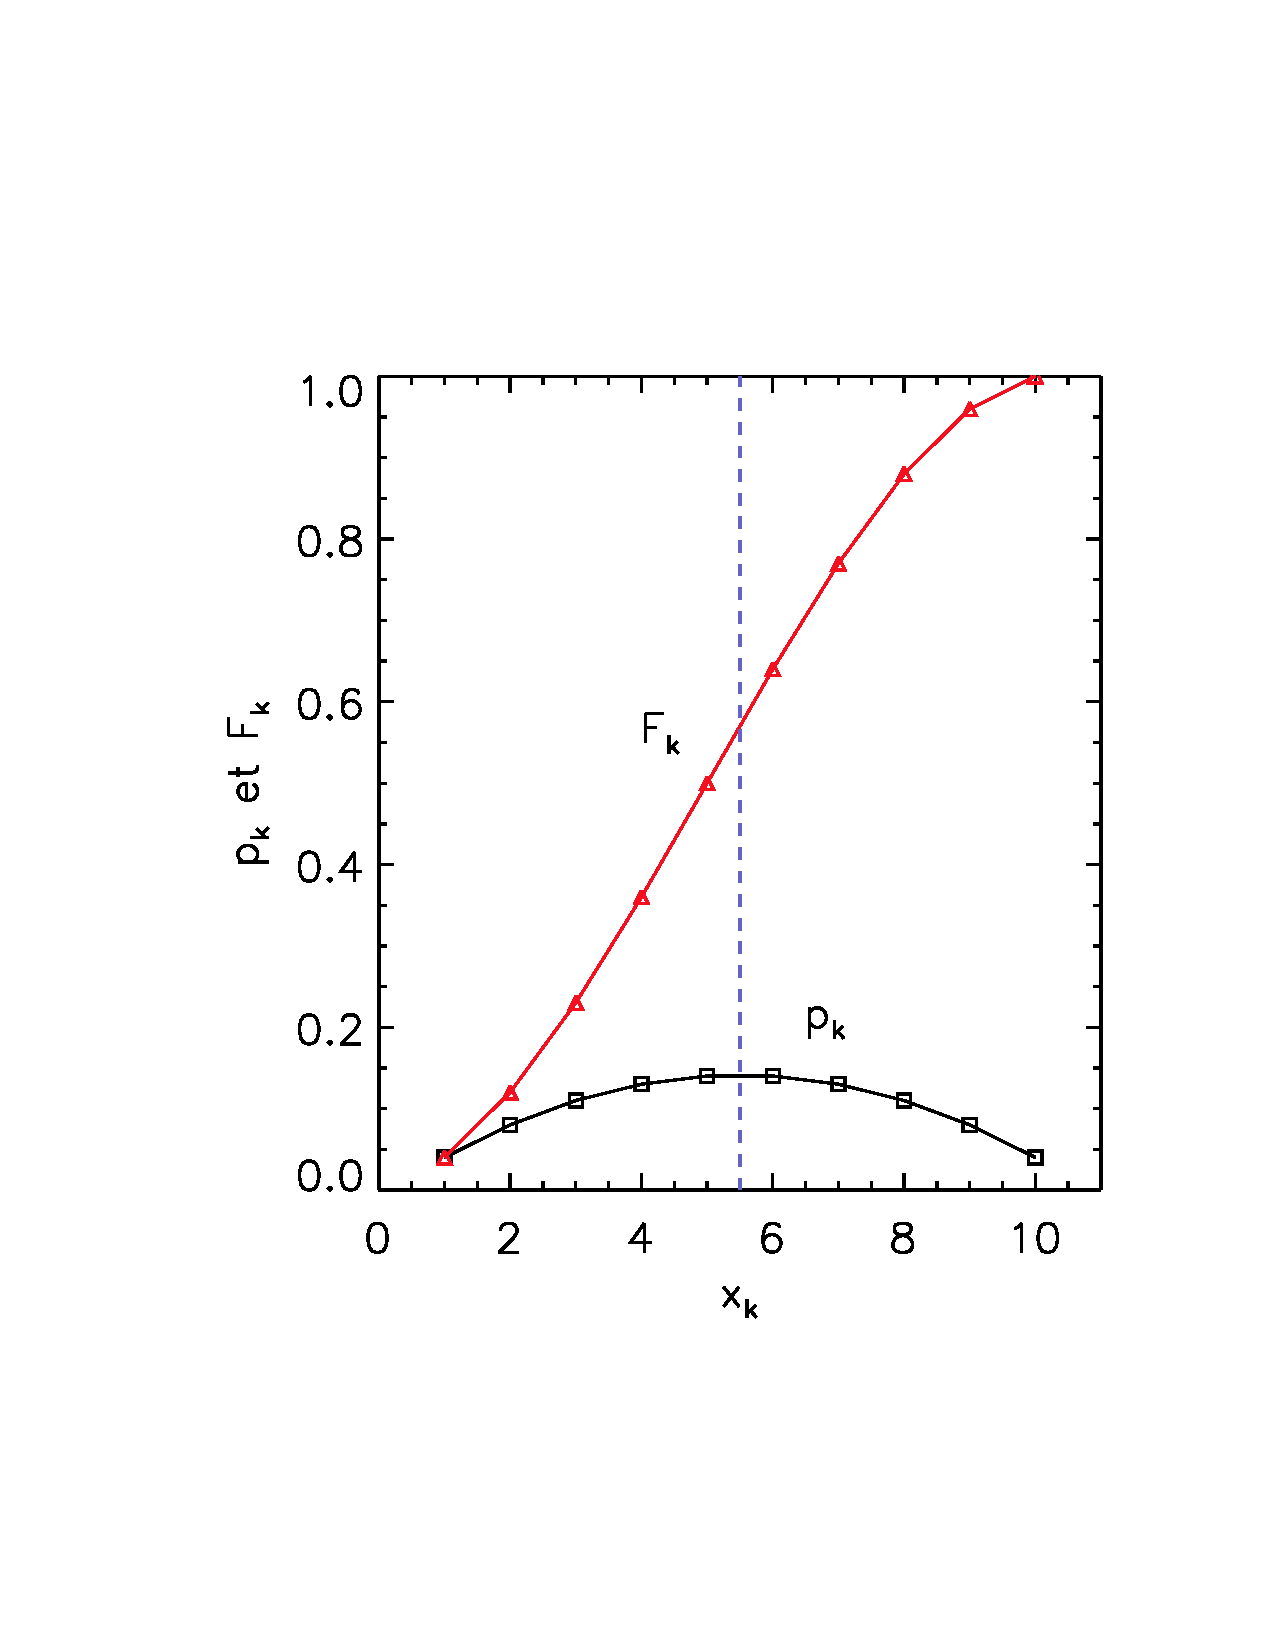
\includegraphics[width=6.5cm]{assets/figures/probabiliteEtfonctiondeRepartition.pdf}
   \caption{Distribution de probabilité de l'exemple des 100 mesures (courbe noire). En rouge, la fonction de répartition. La médiane est égale à la moyenne et vaut 5.5.}
   \label{fig:edfdr}
\end{wrapfigure}

ce qui peut s'écrire, en notation plus compacte, comme la somme
\begin{equation}
\langle x\rangle=\frac{\sum_{k=1}^{10}f_k\,x_k}{N_m}=\sum_{k=1}^{10}p_k\,x_k=5.5
\end{equation}
On voit alors que la moyenne se calcule comme la somme des valeurs de la population, \textbf{pondérées} par leur probabilité d'occurrence. On généralise ce résultat pour toutes les puissances de $x$, en introduisant \textbf{le moment d'ordre $\mathbf{m}$ d'une VA $\mathbf{x}$ discrète}, égal à la moyenne de $x^m$:
\begin{equation}
\langle x^m\rangle=\sum_{k=1}^{N_p}p_k\,x_k^m
\end{equation}

\noindent\textbf{La moyenne simple} est donc donnée par
\begin{equation}
\langle x\rangle=\sum_{k=1}^{N_p}p_k\,x_k
\end{equation}

\textbf{L'écart quadratique moyen} est donné par
\begin{equation}
\text{EQM}(x)=\langle (x-\langle x\rangle)^2\rangle=\langle x^2\rangle-\langle x\rangle^2=\sum_{k=1}^{N_p}p_k\,x_k^2-\left(\sum_{k=1}^{N_p}p_x\,x_k\right)^2
\end{equation}
que l'on appelle aussi la variance, et \textbf{l'écart-type} est simplement
\begin{equation}
\sigma(x)=\sqrt{\text{EQM}(x)}
\end{equation}

\subsection{Fonction de répartition d'une variable aléatoire discrète}

La somme partielle
\begin{equation}
F_k=\sum_{l=1}^{k} p_k=P[x\le x_k]
\end{equation}
définit la \textbf{fonction de répartition} de la VA. On a $F_1=p_1$ et $F_{N_p}=1$, où $N_p$ est la dimension de la population. Voir la figure~\ref{fig:edfdr}, pour la fonction de répartition de l'exemple des 100 mesures précédent. Nous avons aussi vu un exemple de fonction de répartition au premier chapitre, avec la somme partielle des fréquences. À nouveau, la somme partielle des fréquences ne s'identifie à la fonction de répartition que lorsque le nombre de mesures tend vers l'infini.

\subsection{Mode et médiane d'une variable aléatoire discrète}

Le \textbf{mode} de la VA est la valeur de $x$ pour laquelle $p_k$ est maximale, et la \textbf{médiane} la valeur de $x$ qui sépare la probabilité en deux sommes partielles égales:
\begin{equation}
\sum_{k=1}^{k_{\text{med}}}p_k=\sum_{k=k_{\text{med}}}^{N_p}p_k=\frac{1}{2}
\end{equation}
Ici il y a une petite difficulté: il peut se faire qu'aucune valeur de la population $\mathcal{P}$ ne satisfasse à cette définition, c.-à-d. que la valeur de la médiane soit située entre deux valeurs successives de $\mathcal{P}$, comme c'est le cas dans l'exemple ci-dessus: la somme des probabilités entre $x=1$ et $x=5$ est de 0.5, et la somme de $x=6$ à $x=10$ est aussi égale à 5. La médiane est donc située entre $x=5$ et $x=6$, soit, par interpolation $x=5.5$.

\section{Les distributions de probabilité des variables aléatoires continues}

Ce paragraphe constitue un rappel général sur les probabilités des VA continues. Au prochain paragraphe, nous introduirons les distributions continues les plus courantes.

\subsection{La densité de probabilité}

Soit une VA \textbf{continue} x (un nombre réel), mesure d'une grandeur physique $\mathcal{G}$. L'ensemble des valeurs possibles de $x$ est la population $\mathcal{P}$. Cette population est un intervalle continu de valeurs réelles, entre 2 bornes (qui peuvent être infinies). Par conséquent, la dimension de la population d'une VA continue est forcément infinie.

Définir la probabilité de $x$ est ici un peu plus difficile que dans le cas discret. Commençons tout d'abord par diviser la population en un certain nombre de classes (peu importe le nombre) de largeur $\Delta X$. On traite ainsi - momentanément - la VA continue comme une VA discrète. Il est alors possible de définir la probabilité que $x$ appartienne à un intervalle $[X,X+\Delta X]$ par
\begin{multline}
P\{x\in[X,X+\Delta X]\}=\\
\frac{\text{nombre de fois où $x\in[X,X+\Delta X]$ parmi tous les résultats possibles}}{\text{nombre de résultats possibles d'une expérience}}
\label{eq:ddlppuvac}
\end{multline}
Définissons alors la \textbf{densité de probabilité} de la VA $x$ par
\begin{equation}
p(x)=\lim_{\Delta X\rightarrow 0}\frac{P\{x\in[X,X+\Delta X]\}}{\Delta X}
\end{equation}
et on remarquera que cette densité de probabilité ressemble à une dérivée. Si $\Delta X$ est assez petit, alors $p(X)\approx p(X\!+\!\Delta X)$ (noté $\overline{p}$), et on aura
\begin{equation*}
P\{x\in[X,X+\Delta X]\}=\overline{p}\,\Delta X
\end{equation*}
Si à présent $\Delta X\rightarrow0$, alors $P\{x\in[X,X+0]\}=\overline{p}\cdot 0=0$, et donc la probabilité que la VA $x$ soit exactement égale à une valeur précise $X$ sera nulle ! Résultat à priori surprenant, car la valeur $X$ existe bel et bien. Cependant, dans la population $\mathcal{P}\in\text{I}\!\text{R}$, il existe un nombre infini de possibilités, et entre n'importe lesquelles des valeurs de $\mathcal{P}$, il existe encore une infinité de possibilités ! C'est du super-infini. Si on effectue une expérience numérique, le nombre de fois où on tombera exactement sur une valeur précise $X$ sera \textit{infiniment plus petit} que le nombre de fois où on tombera sur n'importe quoi d'autre. La probabilité d'une valeur particulière d'une VA continue est donc nulle, même si cela heurte notre intuition.

En revanche, la probabilité que la VA appartienne à un certain intervalle $[a,b]$ n'est pas nulle ! À l'aide de la densité de probabilité, on pourra alors écrire,
\begin{equation}
P\{x\in[a,b]\}=\int\limits_{a}^{b}p(x)\,\text{d}x
\end{equation}
\textbf{On veillera donc à ne pas confondre probabilité et densité de probabilité !}

\subsection{Propriétés de la probabilité continue}

\begin{itemize}
\item si $[a,b]\in\mathcal{P}$, alors $0\le P\{x\in[a,b]\}\le 1$
\item $P[x\in\text{population}]=1$ c.-à-d. $\int p(x)\text{d}x=1$
\item $P\{x\in[a,b]\ \text{ou}\ x\in[c,d]\}=P\{x\in[a,b]\}+P\{x\in[c,d]\}=\int_{a}^{b} p(x)\text{d}x+\int_{c}^{d} p(x)\text{d}x$
\item si x et y sont deux VA continues indépendantes, de densités de probabilité $p_x$ et $p_y$, alors $P\{x\!\in\![a,b]\ \text{et}\ y\!\in\![c,d]\}=P\{x\!\in\![a,b]\}\cdot P\{y\!\in\![c,d]\}=\int_{a}^{b} p_x(x)\text{d}x\cdot\!\int_{c}^{d} p_y(y)\text{d}y$.
\end{itemize}

\subsection{Moments d'une variable aléatoire continue}\label{par:mdvac}

Le moment d'ordre $m$ d'une VA continue est défini par la moyenne de $x^m$, pondérée par la densité de probabilité $p(x)$, sur toute l'étendue de la population $\mathcal{P}$. De manière similaire au cas des VA discrètes, on a
\begin{equation}
\langle x^m\rangle=\int\limits_{\mathcal{P}}p(x)\,x^m\,\text{d}x
\label{eq:mdvac}
\end{equation}

\textbf{La moyenne simple} est donnée par
\begin{equation}
\langle x\rangle=\int\limits_{\mathcal{P}}p(x)\,x\,\text{d}x
\end{equation}

\textbf{L'écart quadratique moyen} ou \textbf{variance} est donné par
\begin{equation}
\text{EQM}(x)=\langle x^2\rangle-\langle x\rangle^2=\int\limits_{\mathcal{P}}p(x)\,x^2\,\text{d}x-\Big(\int\limits_{\mathcal{P}}p(x)\,x\,\text{d}x\Big)^2
\end{equation}
et \textbf{l'écart-type} sera, comme d'habitude
\begin{equation}
\sigma(x)=\sqrt{\text{EQM}(x)}
\end{equation}
à noter que, très souvent, on note la variance par $\sigma^2$.

\subsection{Fonction de répartition d'une variable aléatoire continue}

La fonction de répartition $F(X)$ détermine la probabilité que la VA $x$ soit inférieure ou égale à une certaine limite $X$,
\begin{equation}
F(X)=\int\limits_{\text{min}(x)}^X p(x)\,\text{d}x
\label{eq:ddlfdrpuvac}
\end{equation}
où $\text{min}(x)$ est la plus petite valeur de la VA dans la population $\mathcal{P}$.

Puisque la fonction de répartition est égale à l'intégrale de la densité de probabilité, il vient automatiquement que \textbf{la densité de probabilité est égale à la dérivée de la fonction de répartition}. En effet, si on dérive~(\ref{eq:ddlfdrpuvac}), il vient, avec $P(x)$ la primitive de $p(x)$,
$$
\frac{\text{d}}{\text{d}X}F(X)=
\frac{\text{d}}{\text{d}X}\left[P(X)-P(\text{min}(x))\right]=p(X)
$$

\subsection{Mode et médiane d'une variable aléatoire continue}

Le mode est, comme toujours, la valeur de $x$ associée au maximum de la densité de probabilité $p(x)$. La médiane de la VA - $\text{med}(x)$ - est la valeur de $x$ qui sépare la probabilité en deux valeurs égales, naturellement égales à 1/2,
\begin{equation}
\int\limits_{\text{min}(x)}^{\text{med}(x)} p(x)\,\text{d}x=
\int\limits_{\text{med}(x)}^{\text{max}(x)} p(x)\,\text{d}x=\frac{1}{2}
\end{equation}
Dans le cas d'une VA continue, la médiane est donc définie sans ambiguité.

\section{Distributions de probabilité continues usuelles}

Nous présentons ci-dessous les distributions de probabilité continues que l'on retrouve le plus souvent en pratique. {\bf Dans le cas des VA continues, l'usage prévaut que l'on utilise aussi le terme distribution de probabilité pour désigner ce qui est en fait une densité de probabilité}, et dans ce cours, on utilisera indistinctement un terme ou l'autre - uniquement pour les VA continues, cela va de soi. En général, c'est en analysant qualitativement le processus de la mesure que l'on va pouvoir prédire le type de loi de probabilité auquel on doit s'attendre.

\subsection{La distribution uniforme}

Soit une population $\mathcal{P}$ constituée par l'intervalle $[a,b]$. Si toutes les valeurs de la population sont équiprobables, c.-à-d. si $p(x)$ est une constante $p$, alors on dit que la distribution est uniforme, et on aura
\begin{equation}
\int_a^b p(x)\text{d}x=p\int_a^b\text{d}x=p(b-a)=1\Longrightarrow p=\frac{1}{b-a}
\end{equation}

\subsubsection{Moments, moyenne, variance, écart-type, mode, médiane}

\begin{itemize}
\item \textbf{Le moment d'ordre $m$} est donné par
\begin{equation}
\langle x^m\rangle=\frac{1}{b-a}\int_a^b x^m\text{d}x=
\frac{b^{m+1}-a^{m+1}}{(b-a)(m+1)}
\end{equation}
\item \textbf{La moyenne} est donnée par
\begin{equation}
\langle x\rangle=\frac{b^2-a^2}{2(b-a)}=\frac{(b-a)(b+a)}{2(b-a)}=\frac{b+a}{2}
\end{equation}
\item \textbf{L'écart quadratique moyen} est donné par
\begin{align}
\langle x^2\rangle-\langle x\rangle^2&=\frac{b^3-a^3}{3(b-a)}-\left(\frac{b+a}{2}\right)^2=\frac{b^2+ab+a^2}{3}-\left(\frac{b^2+2ab+a^2}{4}\right)\nonumber\\
&=\frac{(b-a)^2}{12}
\end{align}
\item \textbf{L'écart-type} par
\begin{equation}
\sigma(x)=\frac{b-a}{\sqrt{12}}
\end{equation}
\item \textbf{Le mode} n'est pas défini, tandis que la \textbf{médiane} est égale à la moyenne.
\end{itemize}

\subsection{La distribution de Gauss ou << loi normale >>}

\begin{figure}[h!]
   \centering
   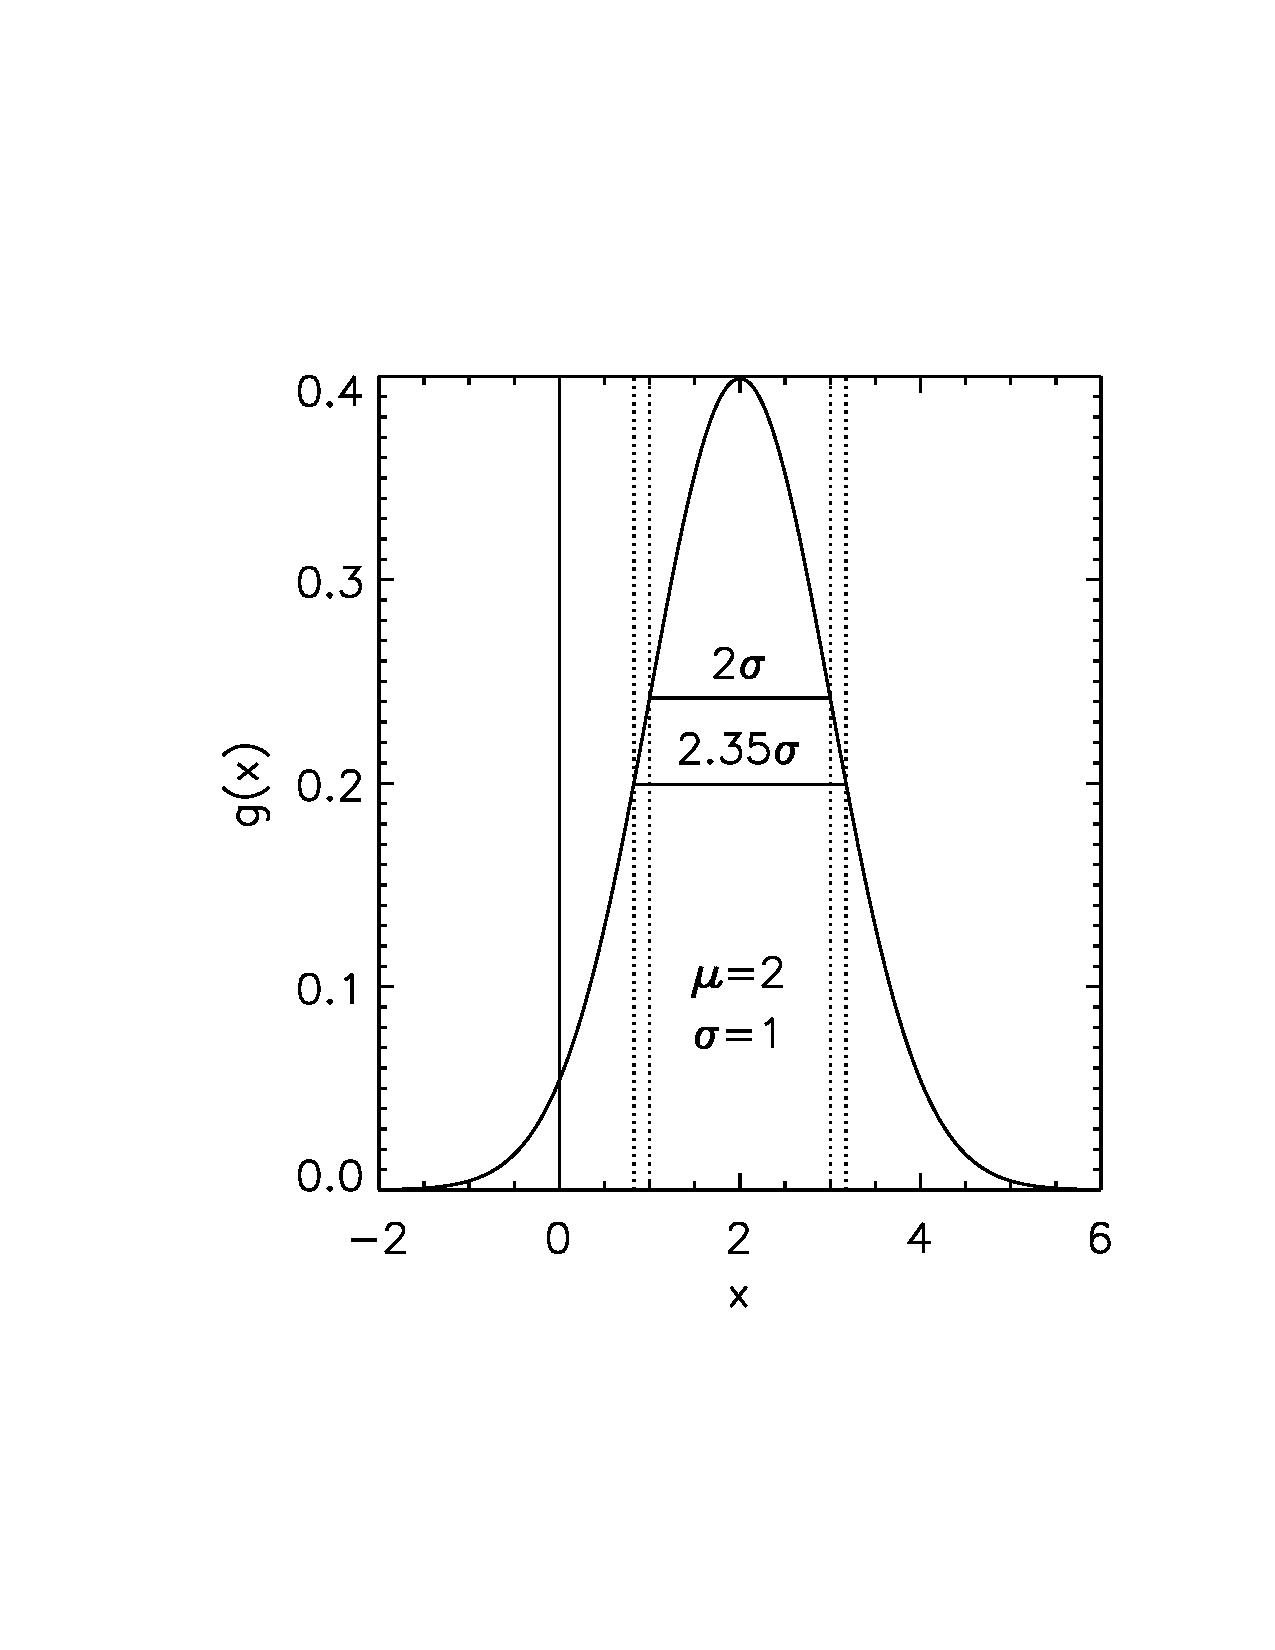
\includegraphics[width=7cm]{assets/figures/loiGaussienne.pdf}
   \caption{Densité de probabilité d'une VA gaussienne de moyenne $\mu=2$ et d'écart-type $\sigma=1$.}
   \label{fig:ddpdlldg}
\end{figure}
La distribution de Gauss\footnote{la courbe dite << en cloche >>} est de loin \textbf{la distribution la plus fréquente rencontrée} lors de la mesure de VA continues. Elle apparait en pratique dans les processus naturels ou techniques qui résultent de la composition d'un grand nombre de processus plus simples et indépendants. Par exemple, dans le cas d'un appareil de mesure complexe - constitué d'un grand nombre de composantes - l'effet total des erreurs individuelles associées à chacune des composantes va se distribuer en général sous la forme d'une courbe de Gauss.

Dans la pratique, très souvent, l'ingénieur fait face à des processus à composantes multiples (les machines construites sont presque toujours des assemblages complexes d'un grand nombre de pièces ou d'éléments), par conséquent on rencontrera, très fréquemment, des VA de type gaussien.

Soit donc X une VA continue de type gaussien, de moyenne $\mu$ et d'écart-type $\sigma$. La densité de probabilité de X est donnée par la formule suivante, que l'on appelle aussi la \textbf{loi normale}
\begin{equation}
g(x)=\frac{1}{\sigma\sqrt{2\pi}}\exp{\left[-\frac{(x-\mu)^2}{2\sigma^2}\right]}
\end{equation}
ou encore la courbe gaussienne, voire parfois tout simplement une << gaussienne >>. On montre en figure~\ref{fig:ddpdlldg} la forme de la loi de Gauss pour une VA de moyenne $\mu=2$ et d'écart-type $\sigma=1$.

\subsubsection{Largeur à mi-hauteur de la courbe de Gauss}

On quantifie souvent la dispersion de la courbe de Gauss par sa largeur à mi-hauteur. On utilise dans la pratique l'acronyme du terme en anglais, soit FWHM pour {\it Full Width at Half-Maximum}. En posant $g(x)/\text{max}(g)=1/2$, on trouve (exercice)
\begin{equation}
\text{FWHM}=2\sqrt{2\ln{2}}\,\sigma\approx2.35\,\sigma
\label{eq:fwhm}
\end{equation}

\subsubsection{Loi normale centrée réduite}

Soit une VA X gaussienne de moyenne $\mu$ et de variance $\sigma^2$. Considérons ensuite la VA Y définie par $Y=(X-\mu)/\sigma$. Cette VA est de moyenne nulle, ce qui est évident, et de variance égale à 1, ce qui est moins immédiat, mais se démontre très simplement en appliquant la définition de l'EQM. On dit alors que cette VA est \textbf{centrée} (de moyenne 0) et \textbf{réduite}, c.-à-d. de variance 1, et sa distribution est donnée par la loi normale dite centrée réduite,
\begin{equation}
g(y)=\frac{1}{\sqrt{2\pi}}\exp{(-y^2/2)}
\end{equation}

\subsubsection{Moments, moyenne, variance, écart-type, mode, médiane}

\begin{itemize}
\item \textbf{Le moment d'ordre} $m$ est donné par la définition habituelle (équation~\ref{eq:mdvac})
\item \textbf{La moyenne} est naturellement égale à $\mu$
\item \textbf{L'écart quadratique moyen ou variance} est donné par $\sigma^2$
\item \textbf{L'écart-type} par $\sigma$
\item \textbf{Le mode} et \textbf{la médiane} sont identiques et donnés par la moyenne $\mu$
\end{itemize}

\subsection{Convergence vers la distribution de Gauss: le théorème central limite}

Considérons un processus complexe, constitué d'un très grand nombre de processus individuels, chacun décrit par une distribution de probabilité \textbf{absolument quelconque}, de type continu ou discret. On peut montrer que si l'effet de ces processus s'additionne, ce qui est très souvent le cas, alors la distribution de probabilité de la VA constituée par l'addition de ces sous-processus sera donnée par la convolution des distributions individuelles.

Or, si on convole entre elles des fonctions de forme quelconque, mais tout de même toujours positive, et tendant vers 0 d'un côté et de l'autre de l'intervalle $]-\infty,+\infty[$, alors on peut montrer que le résultat va tendre vers une courbe gaussienne,
\begin{equation}
f_1(x)\star f_2(x)\star f_3(x)\star\dots\star f_\infty(x)\rightarrow g(x)
\end{equation}
Ce résultat très important en théorie des probabilités est connu sous le nom de \textbf{théorème central limite}. En général, la convergence est obtenue lorsqu'il existe au moins ne dizaine de sous-processus indépendants.

La \textbf{variance globale} de la gaussienne sera donnée par la somme des variances de chaque sous-processus, et la \textbf{moyenne globale} sera égale à la moyenne des moyennes des chaque processus.

\section{Incertitude de la moyenne empirique, intervalle et niveau de confiance}

Nous avons commencé ce chapitre par discuter du fait que la mesure de toute grandeur physique constitue une variable aléatoire, soit parce que la grandeur physique varie par elle-même de manière aléatoire, soit que le processus de mesure soit lui-même source d'erreurs. Souvent, les deux causes interviennent en même temps, mais puisqu'en métrologie nous nous intéressons surtout à la problématique de la précision des mesures, nous allons considérer à partir de maintenant que la fluctuation des mesures est due à la précision limitée des instruments, et que la grandeur à mesurer est, par nature, constante dans le temps.

Nous avons introduit, avec la distribution de probabilité et les moments de la distribution, des outils permettant de quantifier de manière efficace les fluctuations des mesures expérimentales. Parmi ces outils, c'est surtout la moyenne et l'écart-type qui sont le plus largement utilisés, et le résultat d'une mesure est en général annoncé comme suit:
\[
r=\text{moyenne}\pm\text{incertitude}\hspace{2mm} \text{unité}
\]
\textbf{Une question fondamentale se pose alors}: quelle est la fiabilité de la détermination de la moyenne ? Ou en d'autres termes, quel est l'écart probable entre la moyenne empirique, et la vraie valeur de la moyenne - celle que nous cherchons vraiment et que nous trouverions si nous avions une infinité de mesures ? \textbf{Estimer cet écart, c'est estimer la précision de notre mesure !} Examinons cela.

\subsubsection{Incertitude à 1-$\sigma$ sur la moyenne}

Soit donc un échantillon de $N$ mesures, de moyenne et de variance empiriques (c.-à-d. calculées à partir des mesures elles-mêmes, selon les équations des paragraphes~\ref{par:mdvad} ou~\ref{par:mdvac}) données par $\mu$ et $\sigma^2$. Si $N$ était infini, alors la moyenne empirique serait exactement égale à la moyenne de la grandeur physique étudiée. Mais comme $N<\infty$, il existe toujours un écart, inconnu, entre la moyenne vraie et $\mu$, qui n'est qu'une estimation.

On peut facilement montrer\footnote{à l'aide du théorème central limite} que les erreurs sur la détermination de la moyenne se distribuent selon une loi gaussienne, de moyenne égale à $\mu$, et d'écart-type
\begin{equation}
\Delta\mu=\sqrt{\frac{\sigma^2}{N}}=\frac{\sigma}{\sqrt{N}}
\end{equation}
et on voit que cet écart diminue avec le nombre de mesures. $\Delta\mu$ est donc une estimation de l'erreur commise sur le calcul de la moyenne, à partir d'un échantillon de $N$ mesures.

\subsubsection{Intervalle et niveau de confiance à n-$\sigma$}

Pour terminer, il nous faut encore introduire le concept \textbf{d'intervalle et de niveau de confiance} sur l'estimation de la moyenne. Un intervalle de confiance est un intervalle centré sur la valeur moyenne empirique $\mu$ dans lequel on estime que la vraie valeur de la moyenne se trouve avec un niveau de confiance $\alpha$ (entre 0 et 1 - c'est une probabilité).

Sachant que la distribution des erreurs sur la détermination de la moyenne est décrite par une loi gaussienne, on peut calculer les niveaux de confiance (dits à n-$\sigma$) associé aux intervalles $\mu\pm n\Delta\mu$, pour $n=1,2,3\dots$, en intégrant la loi de Gauss sur $[\mu-n\Delta\mu,\mu+n\Delta\mu]$, et on trouve
\begin{center}
\begin{tabular}{r|ccc}
 & 1-$\sigma$ & 2-$\sigma$ & 3-$\sigma$ \\
intervalle de confiance & $\mu\pm\Delta\mu$ & $\mu\pm2\Delta\mu$ & $\mu\pm3\Delta\mu$ \\
niveau de confiance & 68.3 \% & 95.4 \% & 99.7 \%
\end{tabular}
\end{center}

Avec le concept de niveau de confiance, on devra désormais annoncer le résultat d'une mesure de la manière suivante:
\begin{center}
résultat = moyenne $\pm$ incertitude [unité] à $\alpha$ \%
\end{center}
où $\alpha$ est le niveau de confiance associé à l'intervalle moyenne$\pm$incertitude. Par exemple, on dira
$$
m=12.35\pm0.01\ \text{mg}\ \text{à 95 \%}
$$
ce qui signifie que la vraie valeur de $m$ a 95 \% de chances de se trouver dans l'intervalle [12.34,12.36] mg.

Quand on donne un résultat \textbf{sans spécifier} le niveau de confiance, alors par défaut on fera l'hypothèse qu'il s'agit d'un intervalle à 1-$\sigma$, et que donc $\alpha=68.3\,\%$.

\newpage

\section{Exercices du chapitre 7}

\begin{center}
\Large \bf {\underline{Pour faire ces exercices, utilisez \texttt{matlab}}}
\end{center}

\subsection*{Exercice 7.1 - variable aléatoire discrète et distribution de probabilité}

On jette 2 dés à 6 faces. La variable aléatoire à laquelle on s'intéresse est la somme des points sur les deux faces supérieures. Répondre aux questions suivantes :
\begin{itemize}
\item quelle est la population ?
\item quelle est la probabilité $p(v)$ de chaque valeur $v$ ?
\item construire le graphique de la distribution de probabilité
\item quels sont les modes ?
\item quelle est la médiane ?
\item quelle est la moyenne ? visuellement, et avec la formule utilisant $p(v)$
\item calculez l'écart-type, les coefficients d'asymétrie et d'aplatissement
\item quelle est la probabilité que $v\in[\langle v \rangle-\sigma_v,\langle v \rangle+\sigma_v]$ ?
\item prenez deux dés, jetez-les 100 fois, et comparez la distribution des valeurs à ce que vous avez prédit théoriquement.
\end{itemize}

\subsection*{Exercice 7.2 - variable aléatoire discrète}

La variable aléatoire discrète X possède la distribution de probabilité suivante
\begin{center}
\begin{tabular}{c|cccccccccc}
$x_i$    &  -3 &   -2 &   -1 &    0 & 1    & 2    & 3    & 4    & 5   & 6\\
$p_i$ \% & 3.4 & 5.1 & 8.6 & 13.7 & 17.1 & 18.8 & 17.8 & 10.3 & 3.5 & 1.7
\end{tabular}
\end{center}
\begin{itemize}
\item vérifiez que $\sum p_i=1$
\item calculez la moyenne et l'écart-type de X
\item calculez les moments d'ordre 3 et 4
\item donnez le mode
\item calculez la fonction de répartition discrète $F_i$
\item calculez la médiane, par interpolation
\item calculez le niveau de confiance à 1 et 2 $\sigma$, c.-à-d. la probabilité que $X\in[\langle x\rangle\pm\sigma]$ et que $X\in[\langle x\rangle\pm2\sigma]$
\end{itemize}

\subsection*{Exercice 7.3 - variable aléatoire continue}

La mesure d'une tension électrique soumise à des perturbations aléatoires générant une erreur de mesure autour de la valeur moyenne $U_0$ a fourni la distribution de probabilité \underline{continue} suivante
$$
p(U)=\exp{(-2\,|U-U_0|)}
$$
\begin{itemize}
\item vérifiez qu'il s'agit bien d'une distribution de probabilité, c.-à-d. que $\int p\text{d}U=1$
\item calculez la moyenne et l'écart-type de $U$
\item calculez les moments d'ordre 3 et 4
\item donnez le mode
\item calculez la fonction de répartition $F(U)$
\item calculez la médiane
\item calculez le niveau de confiance de l'intervalle d'incertitude à 1, 2 et 3 $\sigma$, c.-à-d. la probabilité que $U\in[U_0-\Delta U,U_0+\Delta U]$ avec $\Delta U=\sigma$, $2\,\sigma$ et $3\,\sigma$)
\end{itemize}

\subsection*{Exercice 7.4 - variable aléatoire continue gaussienne}

\begin{figure}[t]
   \centering
   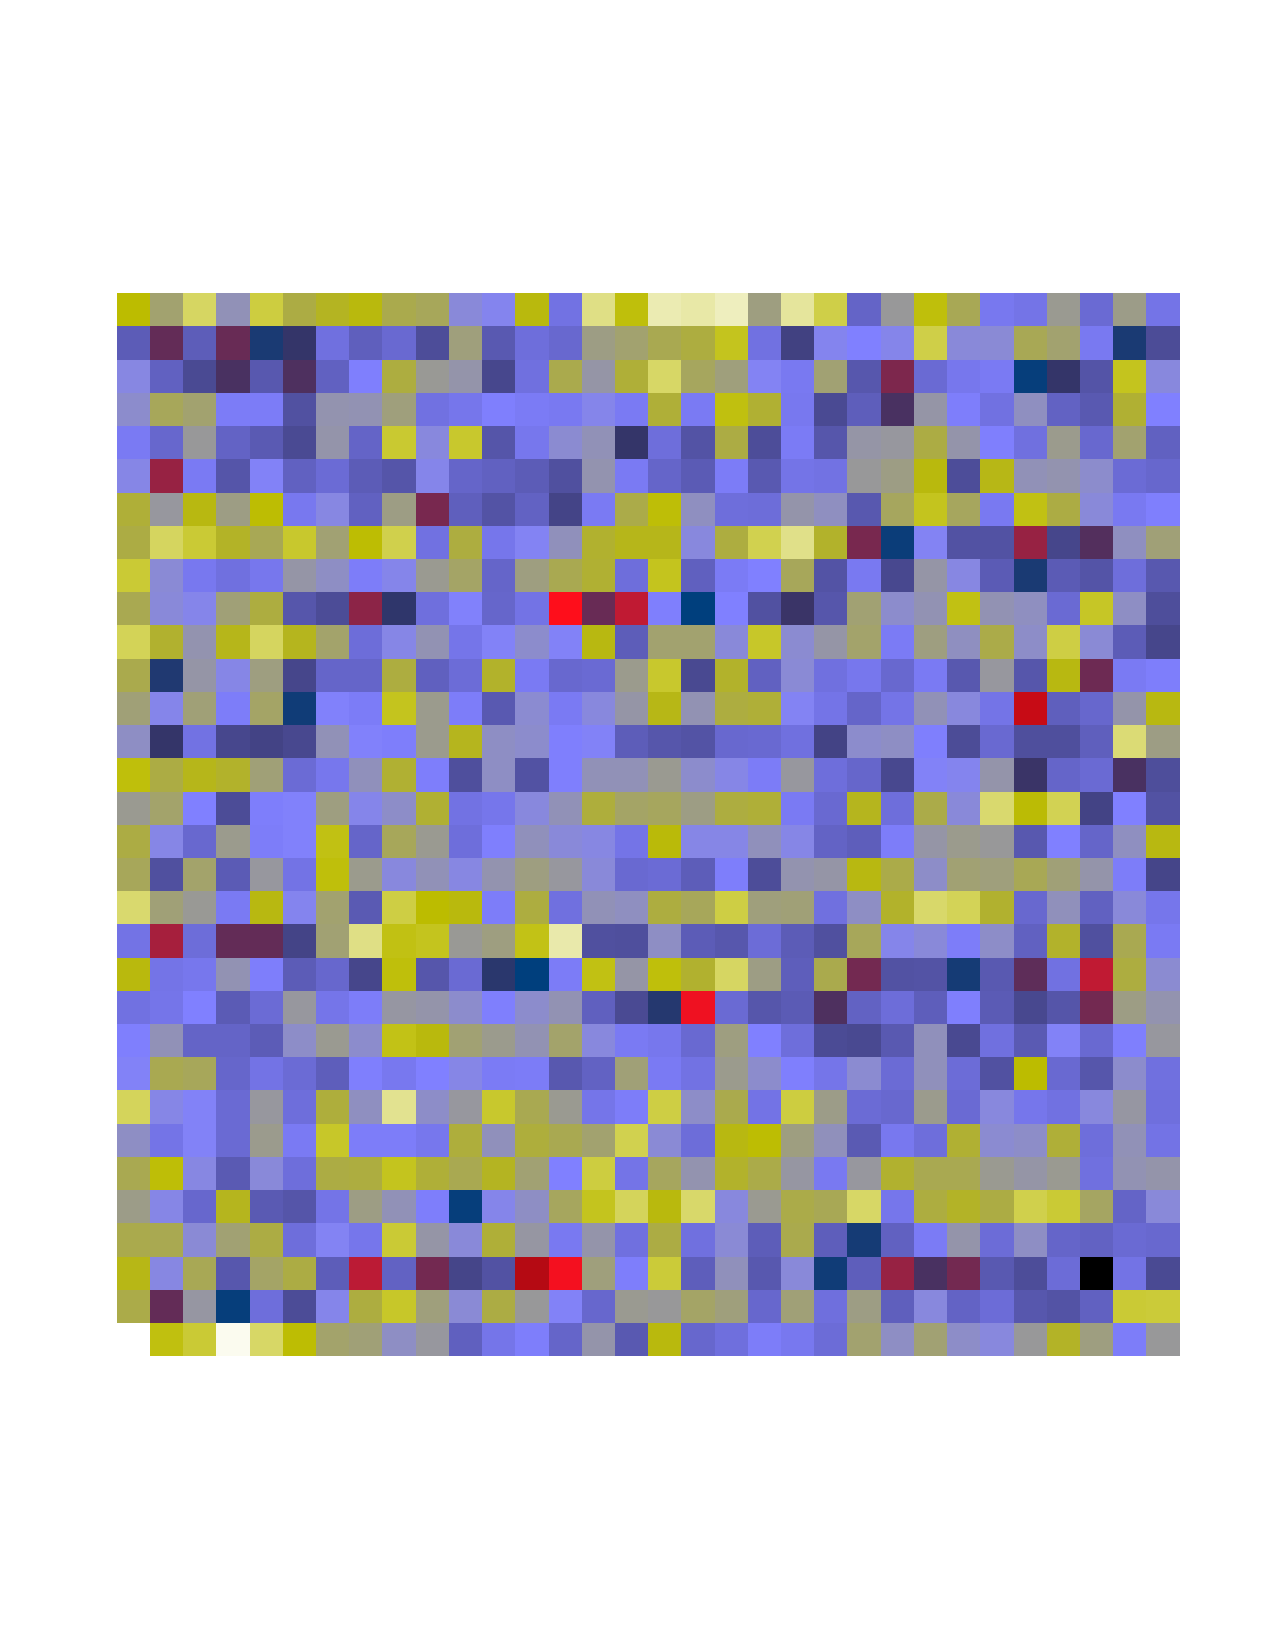
\includegraphics[height=6cm]{assets/figures/Serie2_exe10fig1.pdf}\hspace{10mm}
   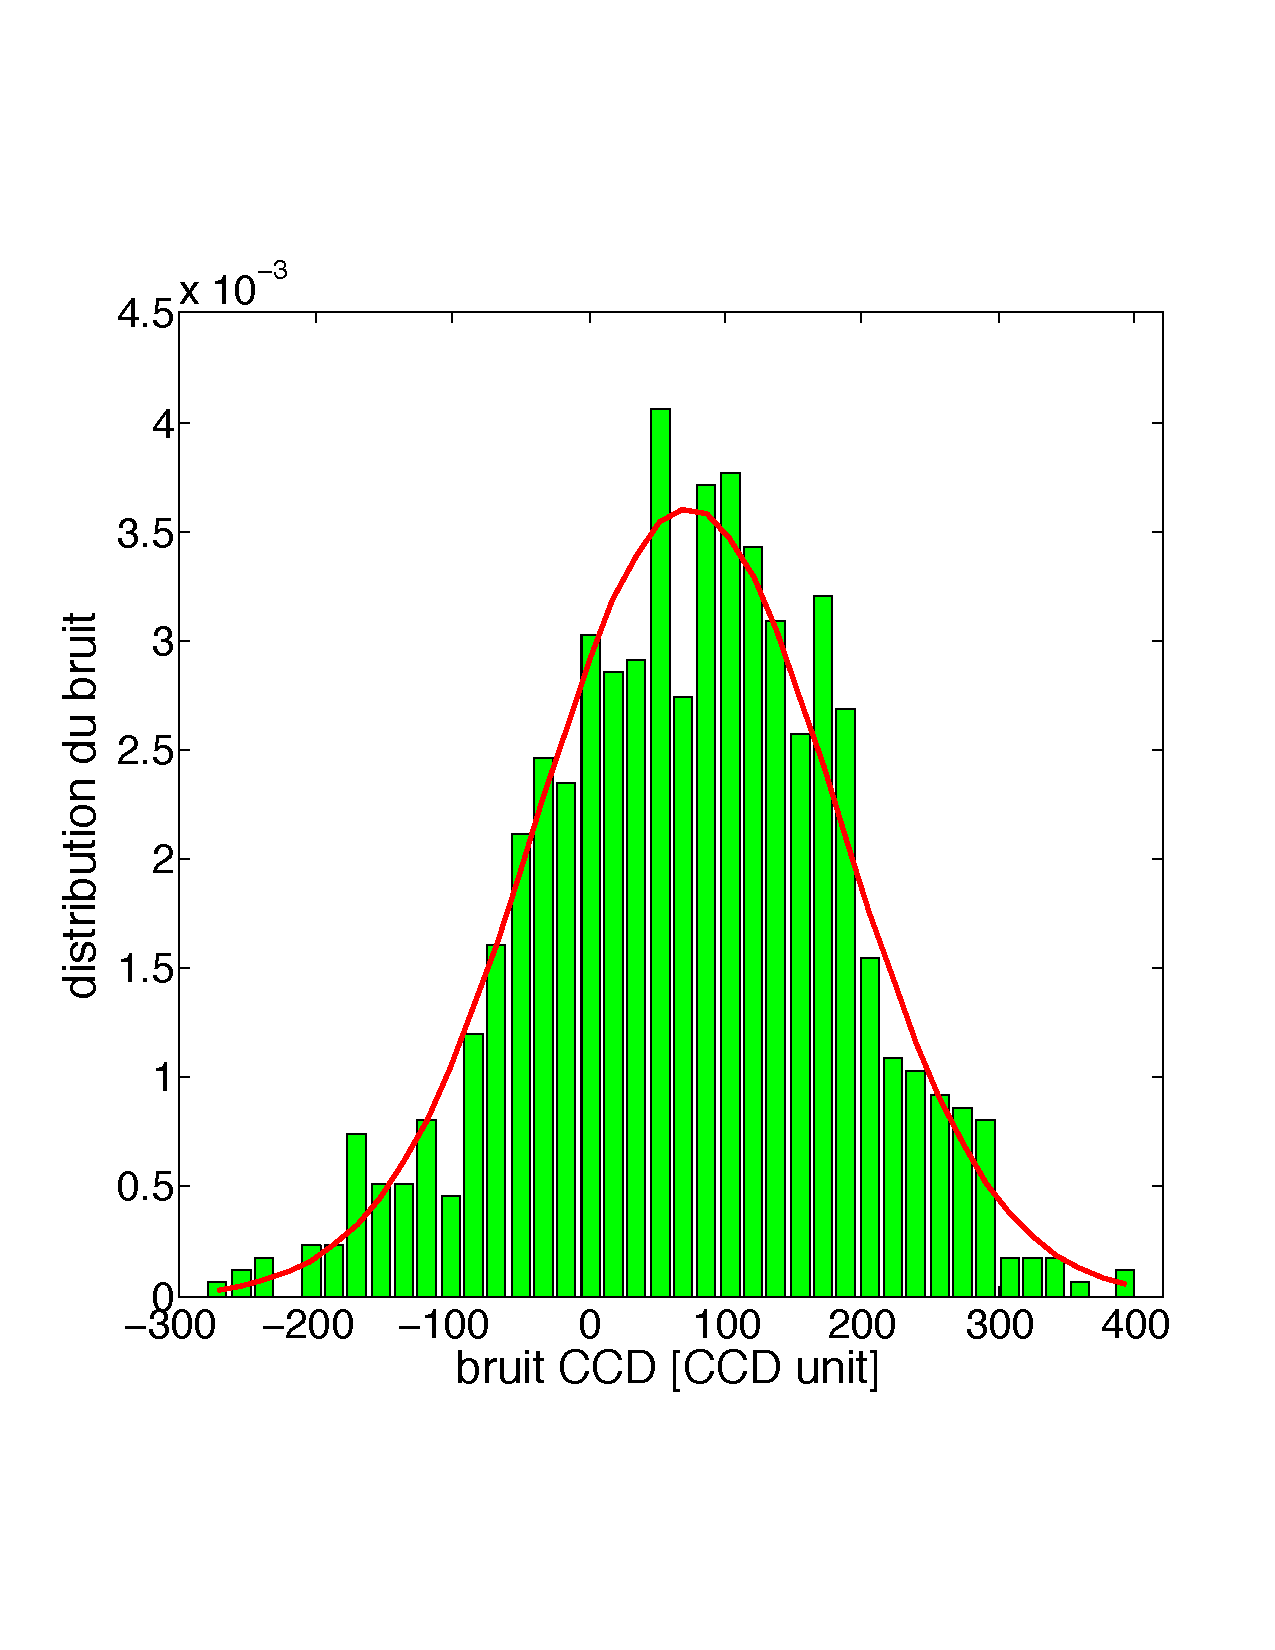
\includegraphics[height=6cm]{assets/figures/Serie2_exe10fig2.pdf}
   \caption{À gauche : détail sur 32x32 pixels du bruit de lecture de la caméra CCD (WMKO); à droite : histogramme des valeurs, avec superposition de la courbe de Gauss correspondant à la moyenne et à l'écart-type mesuré sur l'image.}
   \label{fig:exe16}
\end{figure}

La figure \ref{fig:exe16} (gauche) représente une partie de l'image donnée par un détecteur CCD (détecteur d'image numérique) lors d'une observation stellaire à l'aide du télescope W. M. Keck à Hawaii, USA. Cette partie de l'image ne montre aucune source lumineuse, mais uniquement du bruit de lecture de nature électronique (amplificateur de sortie). L'histogramme des valeurs du bruit est montré dans la même figure, à droite, avec superposition d'une distribution gaussienne de moyenne et d'écart-type égale à celles de l'échantillon, respectivement 73 et 111 photons de bruit.

\begin{itemize}
\item Donnez la valeur moyenne, le mode et la valeur médiane du bruit de lecture, d'après la distribution gaussienne.
\item Calculez la probabilité d'obtenir une valeur positive puis négative de la valeur du bruit.
\item Calculez la largeur à mi-hauteur (notée $\lambda_b$) de la distribution du bruit.
\item Quel est le niveau de confiance de l'intervalle $[\mu_b\pm\sigma_b]$ où $\mu_b$ et $\sigma_b$ sont la moyenne et l'écart-type du bruit ?
\item Et quel est ce niveau pour l'intervalle $[\mu_b\pm\lambda_b/2]$ ?
\end{itemize}
Pour répondre à ces questions, vous pouvez calculez numériquement les intégrales avec \texttt{Matlab}, en approximant les intégrales par des sommes (soit $\int f(x)\text{d}x\approx\sum_if(x_i)\Delta x$), ou alors utiliser \texttt{mathematica}.

\subsection*{Exercice 7.5 - densité de probabilité gaussienne}

Démontrez la formule~\ref{eq:fwhm} de la largeur à mi-hauteur de la distribution gaussienne.

\subsection*{Exercice 7.6 - théorème central limite}

Lancez \texttt{matlab}, définissez un vecteur $x$ de 1000 éléments, et dont les éléments 400 à 600 valent 1, et les autres 0. En utilisant la fonction de convolution de \texttt{matlab}, \texttt{conv()} (voir help), convoluez ce vecteur avec lui-même 1 fois, puis 2 fois, 3 fois, etc. La syntaxe est la suivante:
\begin{verbatim}
>> x=zeros(1000,1);
>> x(400:600,1)=1;
>> y=conv(x,x);
>> plot(y)
>> y=conv(y,x);
>> plot(y)
\end{verbatim}
Répétez les deux dernières lignes un grand nombre de fois. Comment se comporte le résultat de ces convolutions multiples ?

\newpage
\subsection*{Exercice 7.7 - incertitude et niveau de confiance}

On a mesuré 10'000 fois la cote d'une pièce mécanique, et obtenu un écart-type des données de 0.005 mm. Quelle est l'incertitude sur la moyenne, pour un niveau de confiance à 2-$\sigma$ ?

\subsection*{Exercice 7.8 - incertitude et niveau de confiance}

Combien de mesures faut-il effectuer pour s'assurer que, pour l'exemple de l'Exercice 7.15 ci-dessus, l'incertitude à 3-$\sigma$ sur la mesure soit inférieure à 0.001 mm ?